\section{Theoretische Einführung}
\noindent Tomographische Verfahren erlauben es, Strukturen dreidimensional abzubilden.
Die Eingangsintensitäten für die Darstellung stammen dabei beispielsweie von
Teilchen wie Neutronen und Elektronen oder hochenergetischen Röntgen- oder
Gammaphotenen. Je nachchdem, welche Struktur sich zwischen Strahlungsquelle und
Empfänger im Strahlengang befindet, wird die Intensität verschieden stark
abgeschwächt. Die Durchleuchtung der Strukturen aus verschiedenen Richtungen
führt schließlich zu einem richtungsabhängigen Intensitätsprofil, aus welchem
sich die Materialzusammensetzung der Strukturen rekonstruieren lässt. \\
\subsection{Erzeugung der Gammaphotonen}
\noindent Die im Versuch zur Tomographie verwendeten Gammaphotonen entstammen
einer $^{137}Cs$ Strahlungsquelle. Zerfällt eines dieser $^{137}Cs$ Atome, so
geht es zu $\SI{93.5}{\percent}$ in den metastabilen Zustand des $^{137}Ba$
über und zu $\SI{6.5}{\percent}$ in den Grundzustand des $^{137}Ba$ über. Ein
Zerfallsschema des Caesiums ist in Abbildung \ref{fig:01} dargestellt.
\begin{figure}
  \centering
  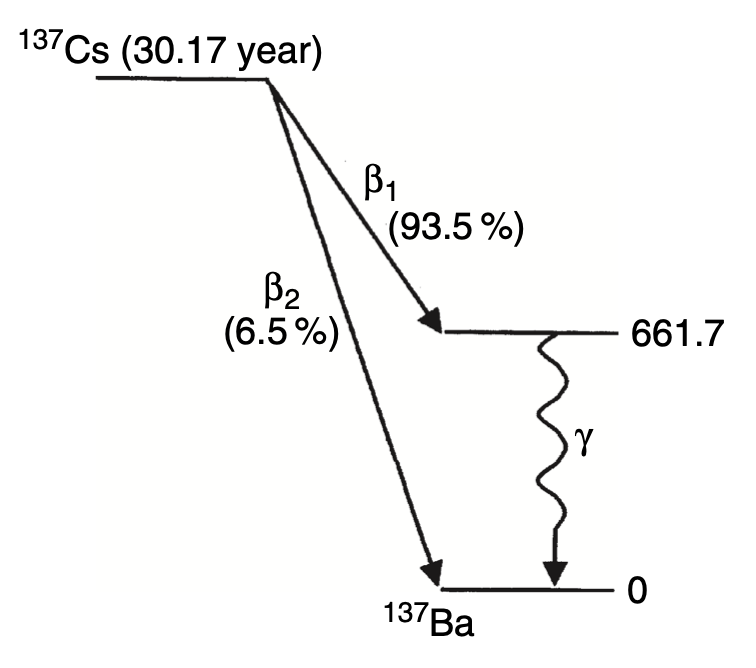
\includegraphics[scale=0.5]{ressources/caesium.png}
  \caption{Zerfallsschema des $^{137}Cs$-Isotops in den metastabilen Zustand des
  $^{137}Ba$ und dessen Grundzustand \cite{gil}.}
  \label{fig:01}
\end{figure}
\noindent Caesium ist ein Betastrahler, der Übergang zum Barium erfolgt durch
Aussendung Umwandlung eines Neutrons unter Aussendung eines Elektrons in ein
Proton. Dadurch erhöht sich die Ordnungszahl des Caesiums um eins und aus dem
Caesium wird Barium. Das ausgehende Elektron wird allerdings im experimentellen
Aufbau abgeschirmt, sodass lediglich das beim Übergang des metastabilen Zustandes
des Bariums in den Grundzustand emittierte Photon zur Tomographie genutzt werden
kann. Die emittierten Photonen haben dabei eine charakteristische Energie von
$E_\text{kin.} = \SI{0.662}{\mega\electronvolt}$, deren Abschwächung beim
Durchdringen verschiedener Materialien Rückschlüsse auf deren Zusammensetzung
erlaubt. \\
\noindent Tritt die emittierte Gammastrahlung mit Materie in Wechselwirkung, so
korelliert die Absorption beim Durchdringen eines Materials mit der Energie der
Photonen. Den Energiebereichen lassen sich dabei drei Effekte zuordnen, welche
die charakteristischen Absorbtionen beschreiben. \\
\subsubsection{Compton-Streuung}
\noindent Für Energiebereiche, in denen die Bindungsenergie der Elektronen im
untersuchten Material klein gegenüber der Energie der Gammaphotonen ist, kann
das Elektron als freies Elektron genähert werden. Der Zusammenstoß zwischen
Elektron und Photon ist inelastisch und es gilt Impulserhaltung zwischen den
Stoßpartnern. Durch den Stoßvorgang gibt das Photon einen Teil seiner
kinetischen Energie an das Elektron ab, der Energieübertrag hängt dabei vom
Streuwinkel zwischen Elektron und Photon ab \cite{demtroeder_3}. \\
\subsubsection{Photoeffekt}
\noindent Ein weiterer Absorptionsprozess für Strahlung, der Photoeffekt, tritt
ebenfalls auf, sobald die Photonenenergie größer als die Bindungsenergie der
Elektronen ist. Diese Bedingung ist für die Gammaphotonen erfüllt. Stößt ein
Photon mit einem der Hüllenelektronen zusammen, so wird dieses aus seiner Hülle
herausgeschlagen. \\
\subsubsection{Paarerzeugung}
\noindent Wechselwirkt ein hochenergetisches Photon, dessen Energie mindestens der
Summe der Ruheenergien von einem Positron und einem Elektron entsprechen muss,
in der Nähe des Atomkerns mit dem Coulomb-Feld des Atoms, so zerstrahlt es dort
zu einem Elektron-Positron-Paar. Die Summe der Ruheenergien von Positron und
Elektron beträgt $2 \cdot m_e \cdot c^2$ (mit Elektronenmasse $m_e$ und der
Lichtgeschwindigkeit $c$), ein Energiebetrag, welchen die im Versuch emittierten
Gammaphotonen nicht erreichen, weshalb dieser Prozess im Experiment
vernachlässigt werden kann. \\
\newline
\noindent Ein exemplarischer Verlauf der energieabhängigen Absorption ist in
Abbildung \ref{fig:02} gegeben.
\FloatBarrier
\begin{figure}
  \centering
  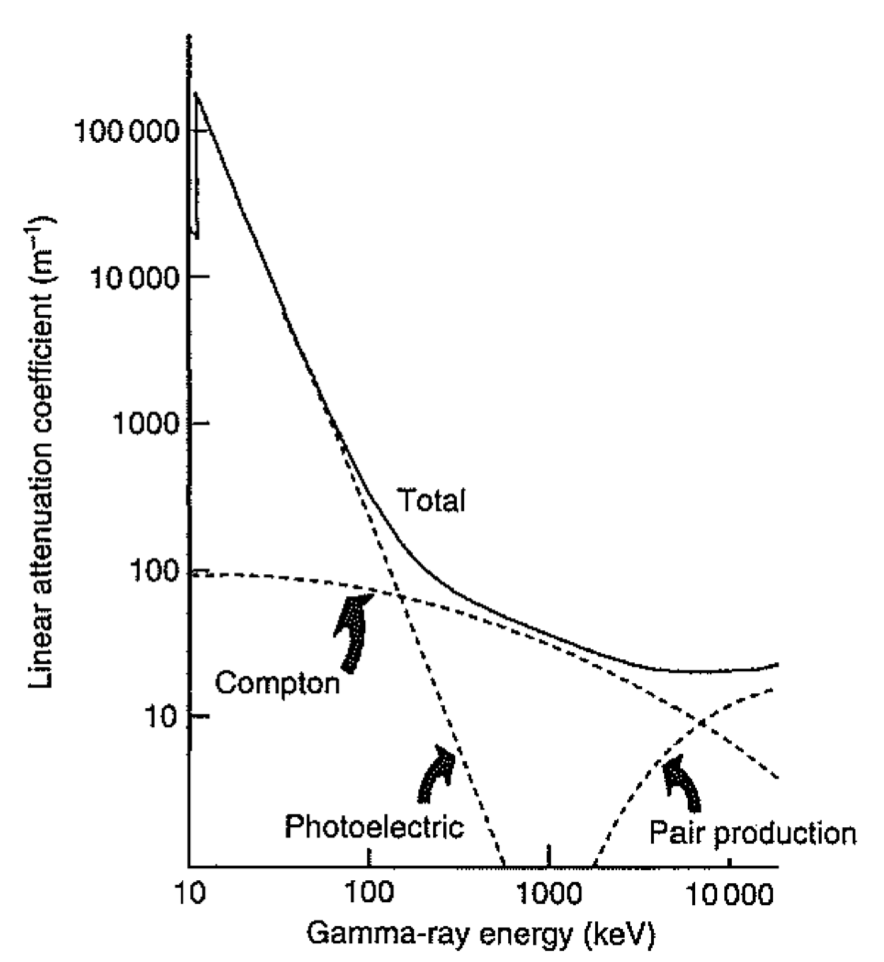
\includegraphics[scale=0.5]{ressources/abschirmung.png}
  \caption{Energieabhängige Absorption von Strahlung am Beispiel Germanium
           \cite{gil}.}
  \label{fig:02}
\end{figure}
\FloatBarrier
\noindent Die zur Tomographie genutzten Gammaphotonen wechselwirken mit ihrer
Energie von etwa  $\SI{0.662}{\mega\electronvolt}$ überwiegend durch
Compton-Streuung mit den Absorbermaterialien, zu einem geringen Teil jedoch auch
über den Photoeffekt.
\subsection{Absorption der Gammaphotonen}
Die vom Caesium-Substrat emittierten Photonen treffen auf ihrem Weg zum Detektor
auf das zu untersuchende Material. Innerhalb des noch unbekannten Materials
wechselwirken die Gammaphotonen mit den Elektronen des Materials im Strahlengang
und werden dort teilweise absorbiert. Für das am Detektor eingehende Signal gilt
daher der Zusammenhang
\begin{align}
  I(d) = I_0 \cdot \exp{(- \mu \cdot d)},
  \label{eqn:01}
\end{align}
wobei $I_0$ der Strahlungsintensität des Caesium-Substrats entspricht, der
Faktor $d$ der Wegstrecke im absorbierenden Material und $\mu$ dem
materialspezifischen Absorptionskoeffizienten. Der Exponent der Gleichung
\ref{eqn:01} muss für den vorliegenden Versuch allerdings dahingehend ergänzt
werden, dass sich auch verschiedene Absorbermaterialien hintereinander befinden
können und ist daher als Summe von Produkten verschiedener
Absorptionskoeffizienten mit den jeweiligen Materialstärken zu beschreiben. Es
gilt folglich der Zusammenhang
\begin{align}
  I_j = I_0 \cdot \exp{\left(\sum_{i} - \mu_i \cdot d_i \right)},
  \label{eqn:02}
\end{align}
\noindent wobei das $j$ hier ein Index zur genauen Beschreibung der Richtung des
Strahls durch den Würfel ist. \\
\noindent Unter der Annahme gleicher Volumina der jeweiligen Würfelstrukturen
innerhalb des Würfels lassen sich die Strecken $d_i$ ermitteln. Die
Materialzusammensetzung ergibt sich daher aus der Summe der
verschiedenen Absorptionskoeffizienten $\mu$. Durch mehrmaliges durchstrahlen
des Würfels aus verschiedenen Richtungen ergibt sich ein überbestimmtes
Gleichungssystem, welches genutzt werden kann, um die Absorptionskoeffizienten
und damit die Materialien innerhalb des großen Würfels zu bestimmen. \\
\noindent Die verschiedenen Orientierungen des Strahls von Gammaphotonen durch
den Würfel lassen sich mathematisch als Matrix beschreiben. Für eine Matrix $A$
berechnet sich die Gesamtintensität der Gammastrahlung aus dem Produkt von $A$
mit einem Vektor $\vec{\mu}$, welcher die Absorptionskoeffizienten $\mu_i$ der
einzelnen Materialien beinhaltet. Es gilt
\begin{align}
  \textbf{A} \cdot \vec{\mu} = \vec{I}.
  \label{eqn:03}
\end{align}
  \noindent Um die Elemente $\mu_i$ von $\vec{\mu}$ zu bestimmen, wird die
  transponierte Matrix $A^{T}$ bestimmt und von links in Gleichung \ref{eqn:03}
  heranmultipliziert, er ergibt sich
\begin{align}
  \textbf{A}^{T} \cdot \textbf{A} \cdot \vec{\mu} = \textbf{A}^{T} \cdot \vec{I},
  \label{eqn:04}
\end{align}
\noindent Durch Umstellen der Gleichung folgt daraus eine Gleichung der Form
\begin{align}
   \vec{\mu} = \left(\textbf{A}^{T} \cdot \textbf{A} \right)^{-1} \cdot \textbf{A}^{T} \cdot \vec{I},
  \label{eqn:05}
\end{align}
\noindent welche die Berechnung der jeweiligen $\mu_i$ ermöglicht.
